\documentclass{article}
\usepackage{amssymb}
\usepackage{graphics}
\usepackage{graphicx}
\usepackage{float}
\usepackage{amssymb}
\usepackage{amsmath}
\usepackage[margin=1in]{geometry}


\title{A History of the Mathematics Behind Orbital Mechanics}
\author{Trevor Farrell}
\date{\today}

\begin{document}

\maketitle

The history of orbital mechanics -- and the mathematics behind it -- is a touchingly human one. Its origins doubtless emerged from the moment our first sapient ancestors gazed up upon the perfectly circular Moon in the night sky -- similar in nature to the circular gleam of the Sun. With time, our ingenuity and capacity for pattern recognition would bring us to establishing calendars to mark the days, years, the cycles of the Moon, and the passing of the seasons -- our first means of recording orbital phenomena across our solar system. \\ 

As we improved our methods of making and recording our observations, the practice of modelling our solar system grew from its infancy as a means of speculation, and into a matured field of application through space exploration. Not but a few brief (albeit eventful) centuries after the works of Kepler, Newton, Euler and Gauss, man-made probes would find their way to distant planets, moons, and outside the bounds of the very solar system itself; steps that would pave the way for human feet to stride across the surface of other celestial bodies. \\

Outlined in this paper, we will discuss basic tools of orbital mechanics:

\begin{itemize}
    \item Kepler's laws of orbital mechanics made through observation and statistical data
    \item Newton's proof of Kepler's observations, justified from the laws of motion and gravity
    \item Tsiolkovsky's application of orbital mechanics on space travel
\end{itemize}

\section{On The Imaginatively Curious: Kepler's Speculations}

Johannes Kepler was a dreamer, a mystic, and a speculator – and above all else, a scientist. Kepler was the sort to cling to a theorem on the sole basis that it felt right to him, only to dedicate the next decade of his life towards identifying exactly why he was wrong. It was this persistence he demonstrated that proved to be his greatest strength: every step he took brought him closer to a more refined model of the motions of the planets, and indeed, towards a model of the motion of any two-body problem in orbital mechanics. What had started out as a mere reinterpretation of the Tychonic system – itself, just an egocentric mathematical analog to the fundamental heliocentric model of the Copernican system – would soon turn into a justified reimagining of the nature in which forces act on all cosmic matter. By examining the motion of the planets with a fervent obsession – an obsession he carried over to the statistical data compiled by others, most notably Tycho Brahe – and building heuristic analogies from his observations with magnetism, Kepler compiled his findings in two milestone works: \textit{Astronomia Nova} in 1609, which consisted largely of his own findings from ten years worth of observations of the motions of Mars; and \textit{Harmonice Mundi} in 1619, which consisted largely of his arguments for harmonic and congruent models in geometric and physical phenomena. \\

In \textit{Astronomia Nova}, Kepler outlined his first grand revaluation of classical orbital models through the introduction of his first two laws of orbital mechanics -- the first and foremost assertion being that the orbits of the heavenly bodies followed not circular patterns, nor egg-shaped ovoids, but ellipses. Inspired by the works of William Gilbert and his \textit{De Magnete}, (1600) Kepler humored the notion of some force acting between the Sun and the Earth -- one whose strength diminished in proportion to distance, a presupposition of what would eventually become the well-known inverse square law of gravitational attraction. With trail and error, and through careful measurements of aphelion and perihelion, (lowest and highest point in an orbit) Kepler presented his second law on orbital mechanics -- that planets sweep out equal areas in equal times. Written mathematically, \\

$$ \frac{dA}{dt} = \frac{r^2}{2} \frac{d \theta}{dt} $$\\

Where $dA = \frac{1}{2} \cdot r \cdot rd \theta $ represents the triangular area carved out between a point in the center of the sun connecting the placement of a planet at two distinct points in its orbit, such that $\frac{dA}{dt}$ remains constant. \\ 

And indeed, where it could in fact be justified, Kepler’s speculation in the mystical and musical paid off in full. The maximum and minimum velocity of the Earth indeed varied harmonically by a semitone – a ratio of 16:15 – while Venus wavered by only a diesis – a ratio of 25:24. Saturn’s difference between its maximum and minimum angular velocity relative to the sun is approximately 4:5 – resembling a major third.  The difference for Mars closely resembles a 2:3 ratio – a fifth. \cite{historyofmathematics} Due to the nature of harmonic orbit resonance, the planets of the solar system are inclined by a positive feedback loop towards regularly spaced intervals, as would be the case for harmonic resonance between vibrating strings – a perspective that reaffirmed Kepler’s suspicions when he found the ratio between Saturn’s fastest orbital velocity compared to Jupiter’s slowest resembled a perfect 1:2 ratio – exactly that of an octave. This harmonic model would continue to provide its uses for centuries to come: itself derived from Kepler’s third law, the Titus-Bode law would continue to illustrate a very close approximation of all the sequential celestial orbits, falling just short of Neptune. \cite{physics} \\

 Encouraged by his findings, regardless of its popular reception or the copyright claim's made by Tycho Brahe heirs, \cite{heirs} Kepler continued his hot streak into \textit{Harmonice Mundi}, where he formalized his third and final law of orbital mechanics: the law of orbital period. In his wording, \textit{'The ratio of the square of an object's orbital period with the cube of the semi-major axis of its orbit is the same for all objects orbiting the same primary.'} In modern notation, the orbital period solved for time comes out like the following:\\

$$ T = \sqrt{ \bigg( \frac{4 \pi ^2}{G*m} r^3 \bigg) } $$ \\

Where $G$ is our gravitational constant, $m$ is the mass of the central body, and $r$ represents the semi-major axis of orbit: for circular orbits, this distance would be the radius. \\ 

Kepler was not an especially gifted mathematician. His advancements were slow and arduous, and often marred by innocent enough mistakes. Despite his greater appeals for assistance, he was largely ignored by mathematicians of the time prior to his discoveries, namely Magini, Maestlin, and François Viète. And truthfully, his final revision for his second law was built off of simple errors in the introduction that were remedied by a near-perfect and completely opposite set of errors, rendering his final result quite close to accurate. \cite{sleepwalker} In his own words -- words that ring true for many a frusturated mathematician to this day -- he wrote:

\begin{quote}
    “\textit{If thou art bored with this wearisome method of calculation, take pity on me, who had to go through with at least seventy repetitions of it, at a very great loss of time.”}
\end{quote}

Others would later come to revise and reaffirm his discoveries, vindicating Kepler of his reputation as a astronomer from a time when astronomy and astrology had little material distinction in academia. Perhaps the most notable of those who revisited and codified his findings being Sir Isaac Newton himself -- with Kepler's laws standing in as an example problem for none other than his famous laws of gravity and motion.


\section{Newton's Vindication of Kepler:}

By way of refreshing the reader on Newton's fundamental laws of motion outlined in \textit{Philosophiae Naturalis Principia Mathematica} \cite{newton}:

\begin{itemize}
    \item Every body preserves in its state of being at rest or of moving uniformly straight forward except insofar as it is compelled to change its state by forces impressed 
    \item change in motion is proportional to the motive force impressed and takes place along the straight line in which that force is impressed.
    \item To any action there is always an opposite and equal reaction.
\end{itemize}

No shortage of controversy surrounds Sir Isaac Newton's claim to calculus fame when compared to Gottfried Wilhelm Leibniz. A great deal of this discrepency may be reduced to their respective approaches -- when Newton first published his \textit{Principia} in 1687, he was not foremost concerned with outlining mathematical rigor as much as he was with describing the physical laws manifest in our universe. This becomes abundantly clear starting with Proposition 1, Theorem 1: a precise mathematical derivation of Kepler's second law, roughly as follows: \\

First, let us begin by dividing time into even intervals, and time-stamping the location of the orbiting body across the points of the ellipse. By Newton's first law of motion, a celestial body might be inclined -- in the absence of any external external force -- to continue along on its path of travel along a straight line. Indeed, if one were to imagine the Sun mysteriously disappearing, one could picture the Earth continuing to travel in a line tangent to its former near-circular orbit, described in the diagram by vector $AB$ or $Ac$. \\

However, by the law of parallelogram forces, the sequential vector would represent the synthesis of the tangent line $Bc$ and $BV$, derived from the gravitational pull towards point $S$, the center of mass in the two-body model. The result is the final position $C$ at the end of the second interval of time.

\begin{center}
    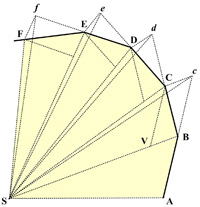
\includegraphics[]{Keplers-Equal-Areas-Law-Newton-Fig.jpg}
\end{center}

And so it would continue for each segment. As Newton observed, each triangular region spanned equal areas for equal intervals of time -- region $BAS$ would equal $CBS$. Furthermore, Newton took an approach not entirely dissimilar to Riemann integration: by increasing the number of time intervals while narrowing each triangular segment arbitrarily, he could demonstrate a continuous curve of constant forces, converging in shape to an ellipse, and acting upon the orbiting object.

\begin{quote}
    \textit{"...Let the number of triangles be increased and their width decreased indefinitely, and their ultimate perimeter will be a curved line; and thus the centripetal force by which the body is continually drawn back from the tangent of this curve will act uninterruptedly, while any area described [BAS, CBS] which are always proportional to the times of description, will be proportional to those times in this case..."} \cite{historyofmathematics}
\end{quote}

But suppose we were to take our fundamental understanding of orbital mechanics and attempt to apply them in a scientific setting. While Kepler’s laws help us understand the path of travel for an object orbiting another in space, what might we use to understand the path it will take were we to impart a force; that is, to change the path of travel?

\section{On The Imaginative Dreamer: Tsiolkovsky and Application of Rocketry In Space Travel}

Konstantin Tsiolkovsky was, by all judgements, a recluse. He preferred to study alone in his log cabin on the far outskirts of his hometown of Kaluga, Russia. Afflicted with near-deafness from scarlet fever contracted at the age of ten, Tsiolkovsky grew up as a shut-in, unable to attain a primary education, and opted instead for a self-taught approach to his studies. \\

And yet, it was in these quieter moments when Tsiolkovsky's true faculties shone brightest. Even as a teenager, enraptured with his math textbooks, he began daydreaming of human space travel and inter-planetary colonization. He is the first human being to seriously conceptualize of the space elevator, upon viewing the construction of the Eiffel Tower in Paris. \cite{elevator} And while he admitted that he never truly expected any of his speculations to come to fruition, this never stopped him from pursuing his studies with the utmost sincerity, stating that his derivations served only as a supplement to philosophical research on the subject.  \\

Perhaps his most widely applicable formulation, written in his namesake, would be the Tsiolkovsky Rocket Equation: \cite{rocket}

$$ \Delta v =  I_{sp} * 9.81 m/s^2 * ln \Bigg( \frac{m_i}{m_f} \Bigg)  $$ 

Where $I_{sp}$ stands for specific impulse, -- multiplied by gravity to form the velocity of the engine's exhaust, and a measure of a rocket engine's efficiency -- $m_i$ stands for initial mass, and $m_f$ stands for final mass. A straightforward means of considering the equation: suppose you were in a single-stage rocket, floating in the middle of deep space, sitting relatively motionless to some starting line. If one were to floor the gas pedal and never let up, just how fast would your rocket be travelling by the time the fuel tank was completely empty? Tsiolkovsky argues that the final result would be dictated by the efficiency of the engine multiplied by the log of the ratio of wet mass to dry mass. \\

A brief derivation is as follows: \cite{rocket} from the perspective of an outside observer, the velocity of the exhaust $V_e$ relative to velocity of the rocket compared to the velocity of the exhaust from \textit{the frame of reference from the rocket} is as follows: \\

$$ V_e = V - v_e \ , \ P= m* \Delta v - v_e * \Delta m $$\\

Where $P$ represents the momentum at time $t = \Delta t$ for our rocket in motion. Since the change in our mass is always negative, (our rocket only expends fuel) and since the sum of our forces meets equilibrium, $\sum F = 0$, we can solve for the first derivative of velocity, using Newton's second law, $F=ma$ as follows: \\

$$ -m \frac{dV}{dt} = v_e \frac{dm}{dt} $$ \\

where assuming $v_e$ is a constant, and integrating using the fundamental theorem of calculus, we achieve \\

$$ - \int^{V+\Delta V}_{V} dV = v_e \int^{m_f}_{m_0} \frac{dm}{m} \Longleftrightarrow \Delta V = v_e ln \Bigg( \frac{m_0}{m_f} \Bigg) $$ \\

As desired. Naturally, this derivation came with a variety of implications. Above all else, this logarithmic relationship demonstrated the need for an exponentially larger rocket in order to make a linear advance in change of velocity. This 'tyranny of the rocket equation' would become the driving motive behind multi-stage rocket designs, and a motivator for more efficient propulsion methods. Through use of its derivation, Tsiolkovsky also found the minimum horizontal velocity necessary to attain a minimal circular orbit around Earth, and with it, discovered that it was indeed entirely possible to construct a multi-stage rocket capable of this performance. While Tsiolkovsky remained humble about his results, there would be no denying that a tangible confirmation of the possibility of space travel was of immeasurable significance -- particularly given that the potential was discovered relatively early in the history of powered flight. Tsiolkovsky published his findings in May of 1903 --  Orville and Wilbur Wright would make their first powered flights in December of that year.    \\

\section{Conclusion:}

Although the totality of orbital mechanics -- along with its primary contributors -- is far too comprehensive for an essay of this scope to address to completion, an argument can be made for the sort of mind required to contribute towards developing the fundamental building blocks for its advancement.  Without exception, each of the aforementioned contributors across the centuries remained captivated and motivated by a sense of wonder for the forces that acted upon all of creation. Each remained intently curious and wildly persistent. And not a single one was afraid to pretend, to imagine, and to dream about the nature of a universe far greater than what simple eyes and ears could hear and see. \\

The mathematics behind mankind's exploration of the cosmos has indeed evolved to a point of complexity far surpassing what might be expected from astrological speculation. And yet there remains not a single step in its journey that hasn't demanded inquiring minds to dream up unique perspectives on ways to interpret reality, such that it fits the numbers we ascribe to our observations. 

\newpage
\bibliographystyle{plain}
\bibliography{bibliography.bib}

\end{document}